\section{Inferencia Bayesiana}
\subsection{Introducción}
\begin{tcolorbox}[colback=blue!5!white, colframe=blue!75!black, title=\textbf{Lo que hemos visto hasta el momento:}]
\begin{itemize}[label=\textbullet]
    \item Se llama el enfoque frecuentista, o clásico de la inferencia.
    \item Hay otro enfoque, llamado la \textbf{inferencia bayesiana}. 
\end{itemize}
\end{tcolorbox}
\begin{tcolorbox}[colback=blue!5!white, colframe=blue!75!black, title=\textbf{La inferencia bayesiana}]
\begin{itemize}[label=\textbullet]
    \item Asume que modelizamos la información que podemos tener sobre el parámetro a través de una distribución de probabilidad.
    \item Formulamos como parte del modelo una \textbf{distribución a priori} sobre $\theta$. Su f.p.p o función de densidad se denota por  $\pi(\theta)$.
    \item La inferencia bayesiana actualiza la información a priori, usando para ello la muestra $\mathbf{x}$ observada, para obtener la \textbf{distribución a posteriori $\pi(\theta|\mathbf{x})$}.
\end{itemize}
\end{tcolorbox}
\subsection{La inferencia bayesiana}
\begin{center}
    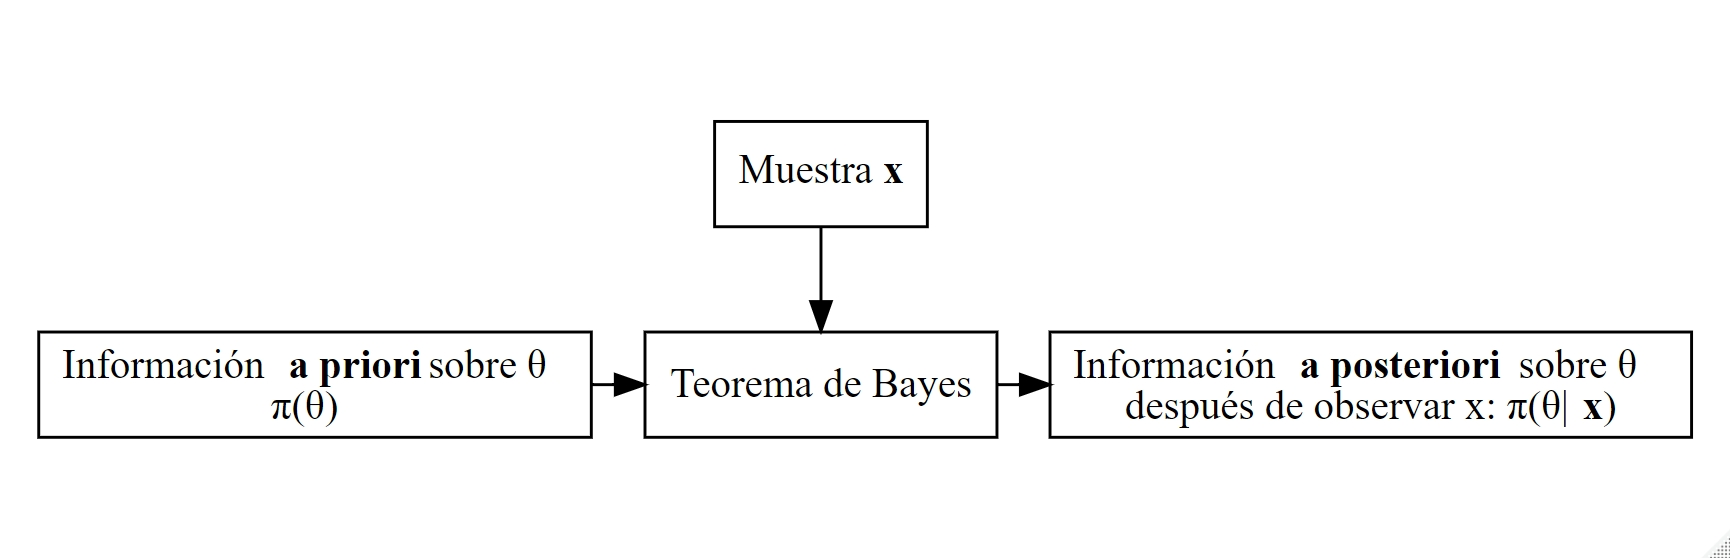
\includegraphics[width=\textwidth]{Tema 5/figures/Figure 1}
\end{center}
\begin{tcolorbox}[colback=olive!5!white, colframe=olive!75!black, title=\textbf{Fórmula de Bayes}]
\[
P(B|A)=\dfrac{P(A|B)P(B)}{P(A)}
\] 
\end{tcolorbox}
\begin{tcolorbox}[colback=blue!5!white, colframe=blue!75!black, title=\textbf{Para distribuciones condicionadas:}]
\[
\pi(\theta|\mathbf{x})=\dfrac{f(\mathbf{x}|\theta)\pi(\theta)}{m(\mathbf{x})},
\] 
\begin{itemize}[label=\textbullet]
    \item $m(\mathbf{x})$ es la marginal de $\mathbf{x}$.
    \item Si $\pi$ es una distribución continua: $m(\mathbf{x})=\int f(\mathbf{x}|u)\pi(u)\du $, la densidad marginal de $\mathbf{x}$ calculada a partir de la conjunta.
    \item Esta integral se realiza sobre el conjunto de valores posibles de $\theta$.
\end{itemize}
\end{tcolorbox}
\subsection{La distribución a posteriori}
En la expresión \[
\pi(\theta|\mathbf{x})=\dfrac{f(\mathbf{x}|\theta)\pi(\theta)}{m(\mathbf{x})},
\] 
$\mathbf{x}$ es el input, una constante. Nos interesa la variable $\theta$, y el denominador solo depende de  $\mathbf{x}$. Escribimos \[
\pi(\theta|\mathbf{x})\propto f(\mathbf{x}|\theta)\pi(\theta),
\] donde $\propto$ quiere decir "es proporcional a".
 \begin{tcolorbox}[colback=olive!5!white, colframe=olive!75!black, title=\textbf{Consejo}]
A veces, será suficiente reconocer el modelo de distribución que sigue $\pi(\theta|\mathbf{x})$ sin tener que calcular el denominador.
\end{tcolorbox}
\subsection*{Ejemplo}
\begin{tcolorbox}[colback=blue!5!white, colframe=blue!75!black, title=\textbf{Ingredientes}]
Lanzamos un dado $n$ veces y apuntamos en cada tirada si ha salido par o impar.
\begin{itemize}[label=\textbullet]
    \item $X\sim \mathrm{Bernoulli}(p),X=1$ si el resultado es par.
    \item muestra: $(x_1,\dots,x_n)$, tenemos que \[
    f(x_1,\dots,x_n|p)=p^{n\overline{x}}(1-p)^{n(1-\overline{x})}.
    \] 
\item Información a priori sobre $p$: puede tomar cualquier valor en $(0,1)$ con igual probabilidad:  \[
\pi(p)=\begin{cases}
    1 & \text{si }p \in (0,1)\\
    0 & \text{en otro caso}
\end{cases}
\] 
\end{itemize}
\end{tcolorbox}
\[
\pi(p|\mathbf{x})\propto p^{n\overline{x}}(1-p)^{n(1-\overline{x})}.
\] 
\begin{tcolorbox}[colback=blue!5!white, colframe=blue!75!black, title=\textbf{Reconocemos una distribución beta}]
Sean dos parámetros positivos $a$ y $b,\,X\sim \mathrm{Be}(a,b)$, si \[
f(x)=\dfrac{\Gamma(a+b)}{\Gamma(a)\Gamma(b)}x^{a-1}(1-x)^{b-1},\text{ para todo $x \in (0,1)$, }
\] siendo $\Gamma$ la función gamma.
 \begin{itemize}[label=\textbullet]
     \item Su esperanza: $E[X]=\dfrac{a}{a+b}$ 
     \item Su varianza: $\mathrm{Var}[X]=\dfrac{ab}{(a+b)^2(a+b+1)}$.
     \item Incluye la distribución uniforme en $(0,1)$, si  $a=1$ y  $b=1$.
     \item En  \lb{\textbf{\texttt{R}}}, \lb{\textbf{\texttt{dbeta}} }, \lb{\textbf{\texttt{pbeta}} }, \lb{\textbf{\texttt{qbeta}} }.
\end{itemize}
\end{tcolorbox}
\begin{tcolorbox}[colback=blue!5!white, colframe=blue!75!black, title=\textbf{Tiramos 10 veces el dado, obtenemos 6 vecer un número par}]
\[
\begin{array}{c}
    \pi(p|\mathbf{x})\propto p^{n\overline{x}}(1-p)^{n(1-\overline{x})}.\\
    \pi(p|\mathbf{x})\sim \mathrm{Be}(1+n\overline{x},1+n(1-\overline{x}))
\end{array}
\] 
¿Qué vale $n\overline{x}$? \[
\pi(p|\mathbf{x})\sim \mathrm{Be}(7,5)
\] 
\end{tcolorbox}
\begin{center}
    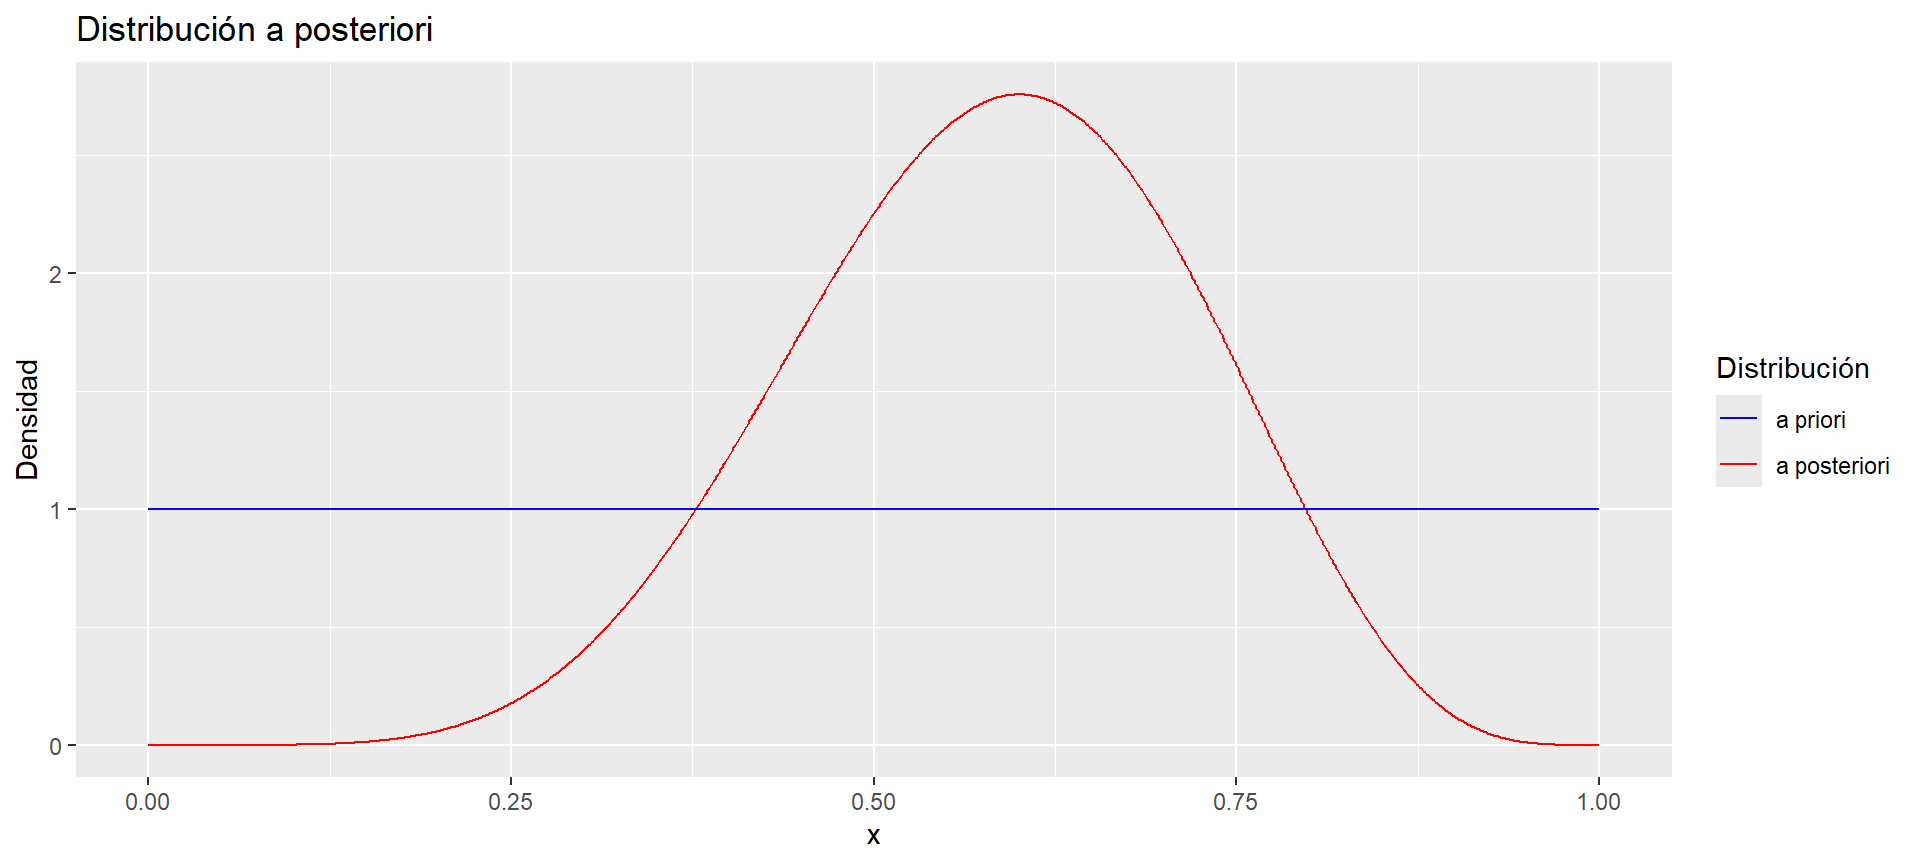
\includegraphics[width=0.7\textwidth]{Tema 5/figures/Figure 2}
\end{center}
Seguimos tirando el dado, hasta 50 veces, obtenemos otras 18 veces un número par, en total 24 veces: $\pi(p)=1,\pi(p|\mathbf{x})\sim \mathrm{Be}(25,27)$ 
\begin{center}
    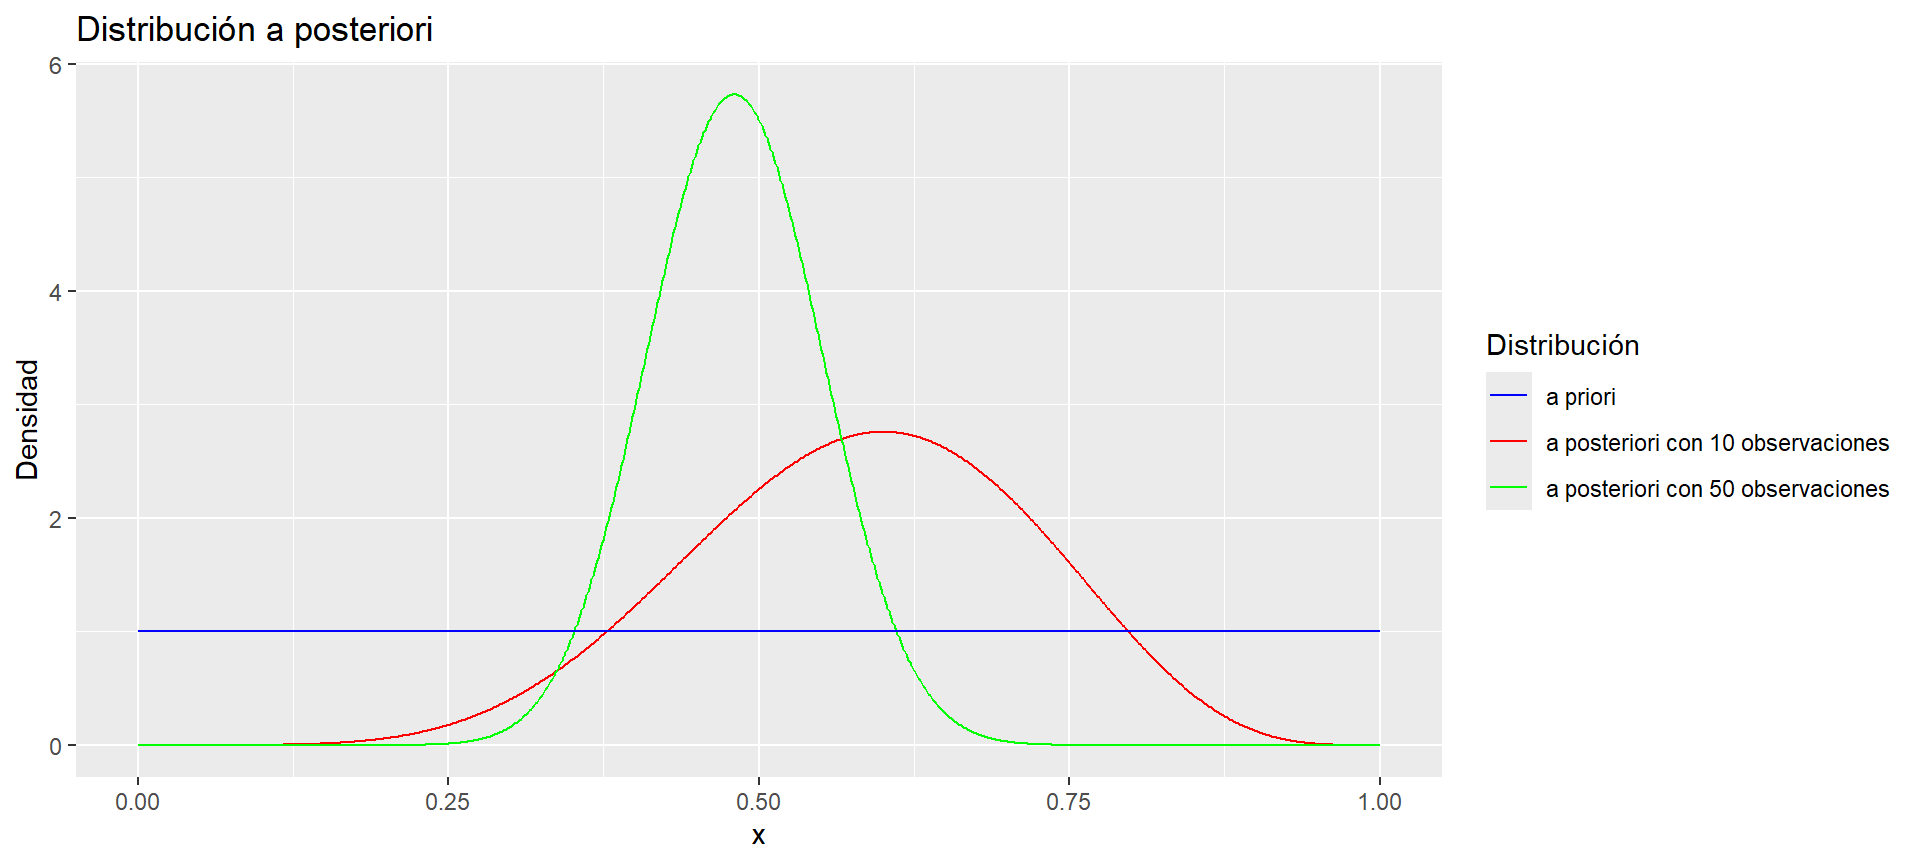
\includegraphics[width=0.7\textwidth]{Tema 5/figures/Figure 3}
\end{center}
\subsection{Distribución a posteriori}
Con el enfoque bayesiando, el resultado de la inferencia, una vez observada una muestra, es una distribución entera, la distribución a posteriori.
\begin{itemize}[label=\textbullet]
    \item Podemos representarla, contiene toda la información que hemos inferido sobre $\theta$, a partir de la muestra y nuestra especificación de la distribución a priori.
    \item Podemos resumirla, por ejemplo con la media, la mediana.
    \item Podemos incluso dar un intervalo que contiene el 95\% de los valores de $\theta$. (\textit{"intervalo de credibilidad al 95\%"} ).
\end{itemize}
\begin{tcolorbox}[colback=blue!5!white, colframe=blue!75!black, title=\textbf{Estimador Bayes}]
Si consideramos una función de pérdida $L(\theta,a)$ asociada a estimar  $\theta$ por  $a$, la pérdida esperada a partir de la distribución a posteriori sería:  \[
    E[L(\theta,a)][\mathbf{x}]=\int_\Omega L(\theta,a)\pi(\theta|\mathbf{x})\dth 
\] para cada valor posible $\mathbf{x}$ del vector aleatorio $\mathbf{X}$, sea $\delta^*(\mathbf{x})$ un valor de a cuya pérdida esperada, dada por la expresión anterior sea mínima. La función $\delta^*(\mathbf{X})$ define un estimado llamado estimador Bayes: \[
\delta^*(\mathbf{X})=\min_{a\in \Theta}E[L(\theta,a)|\mathbf{x}]
\] 
\begin{itemize}[label=\textbullet]
    \item Si $L(\theta,a)=(\theta-a)^2\longrightarrow \delta^*(\mathbf{X})=E(\theta|\mathbf{X})$.
    \item Si $L(\theta,a)=|\theta-a|\longrightarrow \delta^*(\mathbf{X})=$ mediana.
\end{itemize}
\end{tcolorbox}
\subsection*{En el ejemplo de las tiradas de dados}
\begin{minipage}{0.45\textwidth}
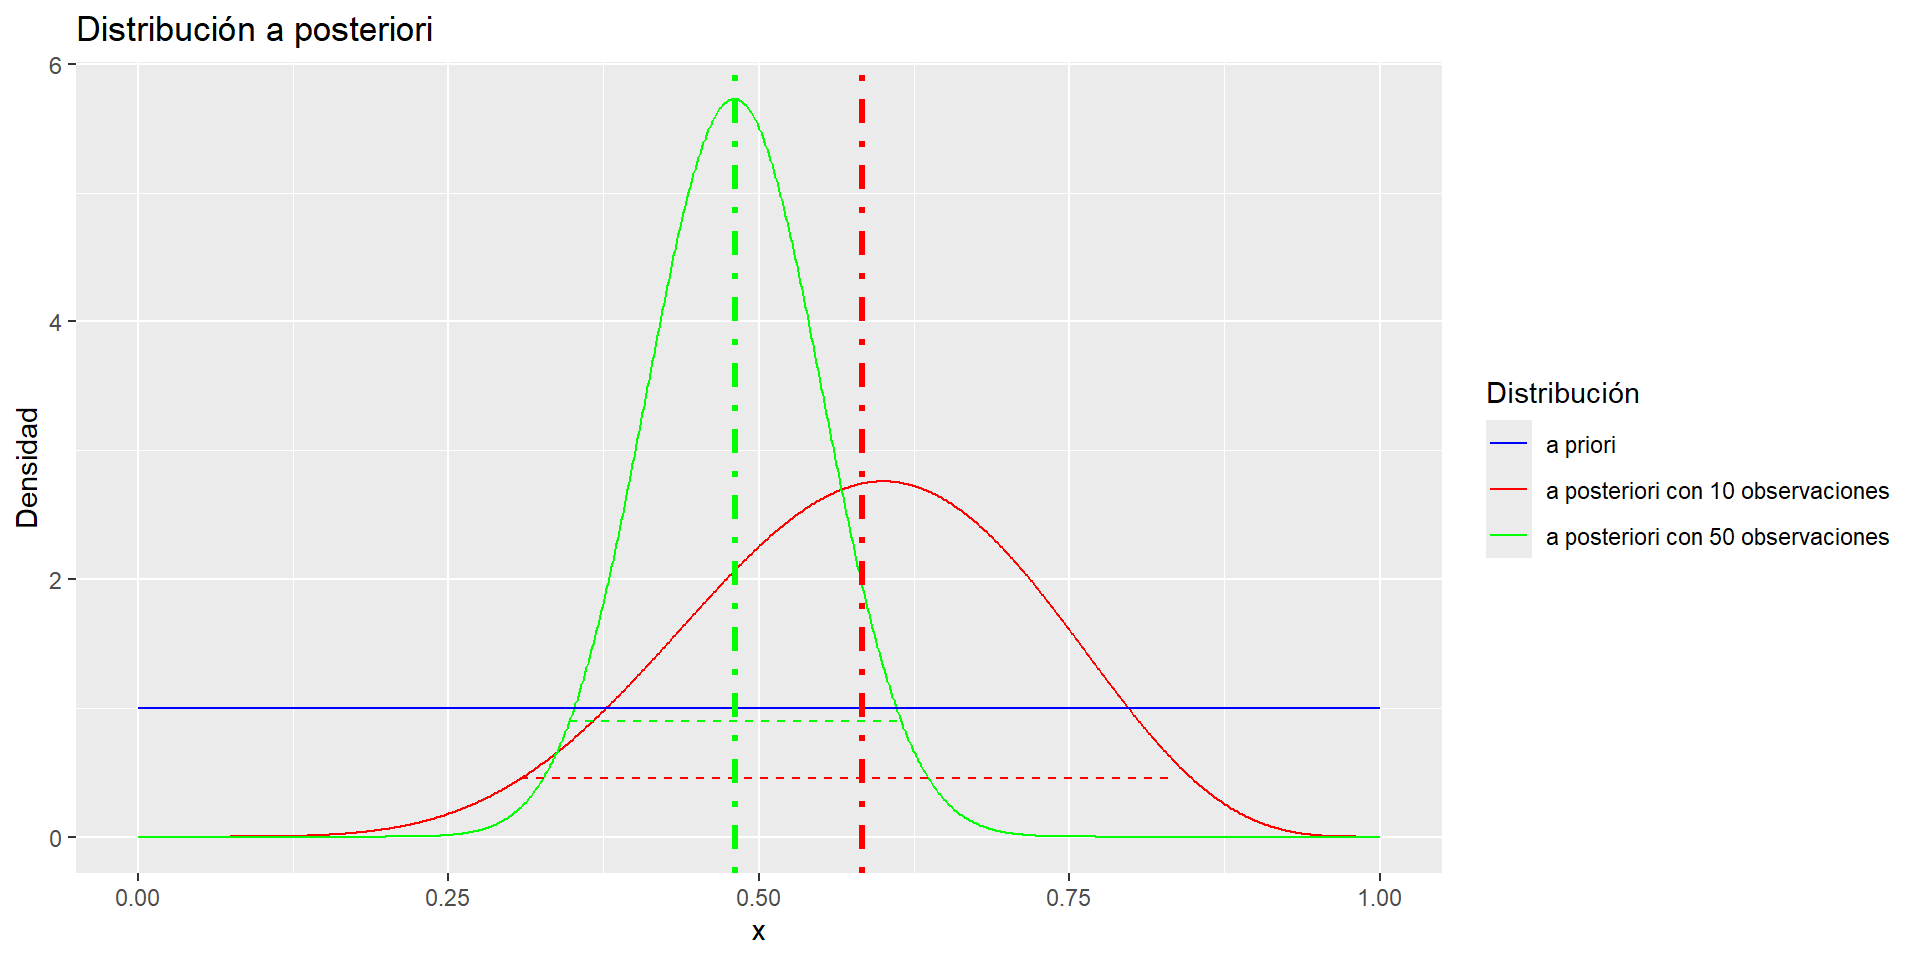
\includegraphics[width=\textwidth]{Tema 5/figures/Figure 4}
\end{minipage} \begin{minipage}{0.59\textwidth}
\begin{tcolorbox}[colback=blue!5!white, colframe=blue!75!black, title=\textbf{Cuando usamos las 10 primeras observaciones }]
\begin{itemize}[label=\textbullet]
    \item $E[p|\mathbf{x}]=\dfrac{7}{12}=0.58$ 
    \item Intervalo credibilidad al 95\%:

        \textbf{\texttt{(qbeta(0.025,7,5),qbeta(0.975,7,5))=(0.31,0.83)}}
\end{itemize}
\end{tcolorbox}
\begin{tcolorbox}[colback=blue!5!white, colframe=blue!75!black, title=\textbf{Cuando usamos las 50 observaciones}]
\begin{itemize}[label=\textbullet]
    \item $E[p|\mathbf{x}]=\dfrac{25}{52}=0.48$ 
    \item Intervalo credibilidad al 95\%:

        \textbf{\texttt{(qbeta(0.025,25,27),qbeta(0.975,25,27))=(0.35,0.62)}}
\end{itemize}
\end{tcolorbox}
\end{minipage}
\subsection{Cambiamos la distribución a priori}
Si $\pi(p)\sim \mathrm{Be}(a_0,b_0)$, y $X|p\sim \mathrm{Bernoulli}(p)$ entonces \[
\pi(p|\mathbf{x})\sim \mathrm{Be}(a'+n\overline{x},b_0+n(1-\overline{x})).
\] 
\begin{tcolorbox}[colback=olive!5!white, colframe=olive!75!black, title=\textbf{Clases conjugadas}]
Decimos que las clase Bernoulli (para $X$) y Beta (para la priori) son \textbf{conjugadas:} la posteriori se queda en la misma clase de distribuciones que la a priori.
\end{tcolorbox}
\subsubsection{La distribución $\mathrm{Be}(a,b)$ es bastante flexible como a priori}
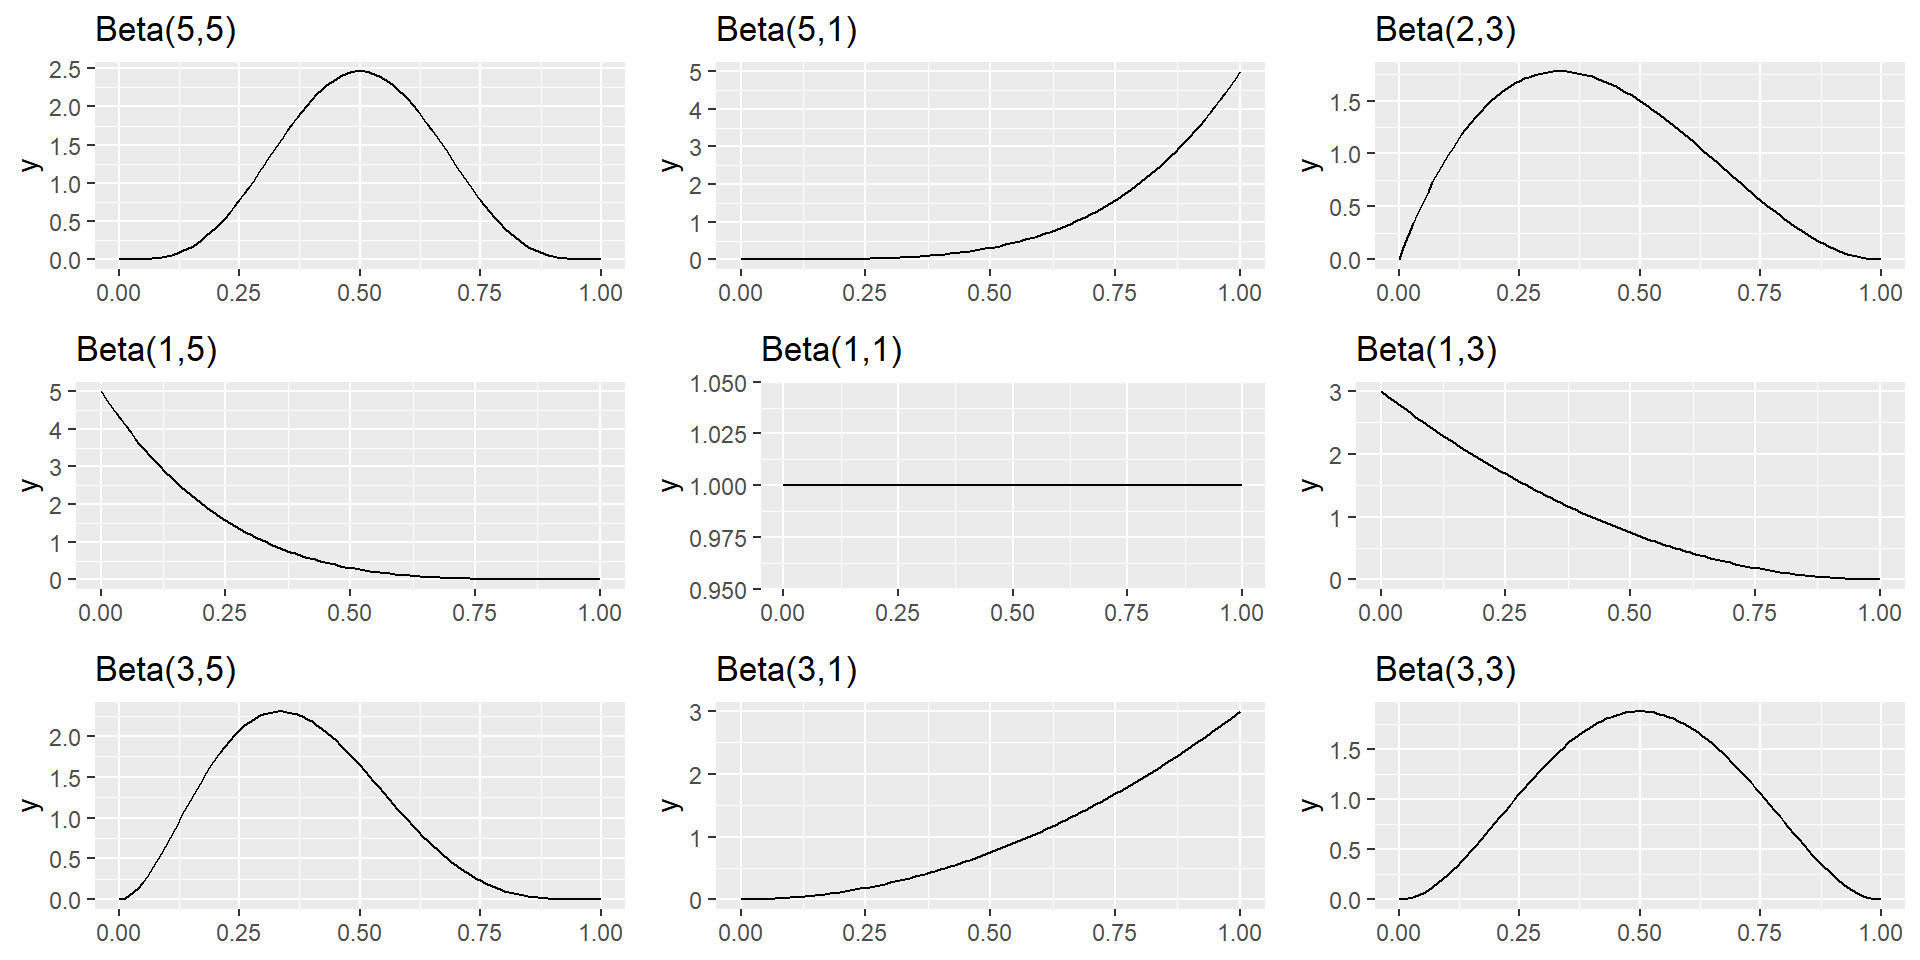
\includegraphics[width=\textwidth]{Tema 5/figures/Figure 5}
\subsection{Aplicaciones de la inferencia Bayesiana}
\begin{tcolorbox}[colback=blue!5!white, colframe=blue!75!black, title=\textbf{La inferencia bayesiana se utiliza en varias áreas del aprendizaje máquina}]
\begin{itemize}[label=\textbullet]
    \item \textbf{Redes Bayesianas} (Belief Networks): Modelos gráficos que permiten representar las dependencias condicionales entre variables aleatorias de forma compacta.
    \item \textbf{Optimización Bayesiana:} Se utilzia para optimizar funciones objetivas que son costosas de evaluar, útil en el ajuste de hiperparámetros para modelos de aprendizaje máquina.
    \item \textbf{Procesamiento de Lenguaje Natural} (PLN): por ejemplo para la clasificiación de texto y el análisis de sentimientos.
    \item \textbf{Sistemas de Recomendación:} Los modelos bayesianos se pueden utilziar para predecir las preferencias de los usuarios y hacer recomendaciones.
\end{itemize}
\end{tcolorbox}
\subsubsection{Ilustración para un ejemplo simple de sistema de recomendación:}
\begin{tcolorbox}[colback=blue!5!white, colframe=blue!75!black, title=\textbf{Contexto:}]
\begin{itemize}[label=\textbullet]
    \item Queremos predecir la probabilidad de que un usuario aprecie una nueva pelicula, para incluirla en las recomendaciones. Sabemos que, entre las 10 películas de este mismo tipo que ha visto, siete le han gustado.
    \item $X\sim \mathrm{Bernoulli}(p):X=1\longleftrightarrow$ "el usuario aprecia una película de este tipo".
    \item Observamos $x_1,x_2,\dots,x_{10}$.
    \item Usamos uan a priori no informativa para $p:\, \pi(p)=\begin{cases}
            1 & \text{si }p\in (0,1)\\
            0 & \text{en caso contrario}
    \end{cases}$
\end{itemize}
\end{tcolorbox}
\[
\pi(p|\mathbf{x})\sim \mathrm{Be}(1+n\overline{x},1+n(1-\overline{x}))\sim \mathrm{Be}(8,4).
\] 
\begin{tcolorbox}[colback=blue!5!white, colframe=blue!75!black, title=\textbf{Inferencia bayesiana predictiva:}]
\begin{itemize}[label=\textbullet]
    \item Tenemos la posteriori $\pi(p|\mathbf{x})$.
    \item Nos interesa $P(X=1|\mathbf{x})$, que es la llamada probabilidad predictiva.
\end{itemize}
\end{tcolorbox}
Para calcularla la obtenemos como marginal usando la posteriori: \[
P(X=1|\mathbf{x})=\int P(X=1|p)\pi(p|\mathbf{x})\mathrm{d}p=\int p\pi(p|\mathbf{x})\mathrm{d}p.
\] 
En este caso: $P(X=1|\mathbf{x})=E[p|\mathbf{x}]=\dfrac{8}{12}=\dfrac{2}{3}$.
\newpage
\begin{center}
    \textbf{\large Hoja de ejercicios Tema 5: Inferencia Bayesiana} 
\end{center}
\begin{enumerate}[label=\color{red}\textbf{\arabic*)}]
    \item \lb{Consideramos el caso en que $X\sim P(\lambda)$ y $\pi(\lambda)$ sigue una distribución gamma con densidad \[
    \pi(\lambda)\propto \lambda^{\alpha-1}\exp\left( -\dfrac{\lambda}{\beta} \right) 
    \]Observamos una m.a.s de $X$, estudiar la distribución a posteriori de  $\lambda$.}
\item \lb{Consideramos una m.a.s. de $X\sim \mathcal{N}(\mu,\sigma^2)$, con $\sigma^2$ conocida y escogemos como distribución a priori $\pi(\mu)$, una distribución normal con densidad \[
\pi(\mu)\propto \exp\left( -\dfrac{1}{2\tau^2}(\mu-\mu_0)^2 \right) 
\]Demostrar que la distribución a posteriori de $\mu$ es Normal con media y varianza: \[
\begin{array}{c}
    E[\mu|x]=\mu_0 \dfrac{\frac{\sigma^2}{n}}{\tau^2+\frac{\sigma^2}{n}}+\overline{x} \dfrac{\tau^2}{\tau^2+\frac{\sigma^2}{n}}\\
    \mathrm{Var}[\mu|x]=\kappa^2=\dfrac{\frac{\tau^2\sigma^2}{n}}{\tau^2+\frac{\sigma^2}{n}}
\end{array}
\] } 
\item \lb{Consideramos una m.a.s. de $X\sim \mathrm{Exp}(1 /\kappa)$. Nota: $\kappa$ es la esperanza de  $X$. Consideramos a priori  $\pi(\kappa)\propto \dfrac{1}{\kappa}$, que se considera una a priori no informativa y es la usual en este caso.}
    \begin{enumerate}[label=\color{red}\textbf{\alph*)}]
        \item \db{Demostrar que la densidad a posteriori de $\kappa|\mathbf{x}$ es proporcional $\kappa^{-n-1}\exp\left( -\sum_{i} \dfrac{x_i}{\kappa} \right) $} 
        \item \db{Demostrar que, si transformamos $\kappa$, considerando  $\lambda=\dfrac{1}{\kappa},\,\lambda|\mathbf{x}$ admite una densidad gamma con parámetros $n$ y $\dfrac{1}{\sum_i x_i}$.}
        \item \db{En un experimento sobre duración de dispositivos, obtenemos los siguientes valores en horas: 6562, 2280, 50, 989, 1797. Obtener un intervalo de credibilidad al 90\% para la inversa de $k$. Obtener el mismo intervalo para  $\kappa$.} 
    \end{enumerate}
\end{enumerate}

